%\documentclass[8pt]{beamer} %with breakpoints
\documentclass[8pt,handout]{beamer} %no breakpoints
\usetheme{Madrid}

\usepackage[utf8]{inputenc}
\usepackage{amsmath}
\usepackage{amssymb}
\usepackage{enumerate}
%\usepackage{mathpazo}
\usepackage{relsize}
\usepackage{mathtools}
\usepackage{verbatim}

\usepackage{tikz}
\usetikzlibrary{matrix,arrows}

\usepackage{commands}

\setbeamertemplate{navigation symbols}{}%remove navigation symbols
%\setbeamertemplate{frametitle}[default][center]

\title{Uhlenbeck compactification as a Bridgeland moduli space}
%\subtitle{Determinantal line bundles on moduli of complexes}
\author{Tuomas Tajakka}
\institute{University of Washington}
\date{October 12, 2020}

\begin{document}

\begin{frame}
    \titlepage
\end{frame}

\begin{frame}{Outline}
    \tableofcontents    
\end{frame}

\section{Dimension 1}
\subsection{Slope stability on a curve}
\begin{frame}[fragile]{Dim 1: Slope stability on a curve}
\begin{columns}[t]
    \column{0.5\textwidth}
    \begin{itemize}
        \item<2-> $C$ a smooth, projective curve over $\C$
        \item<3-> (everything will be over $\C$ - for safety)
        \item<4-> \textbf{Slope} of $E \in \Coh(C)$:
        \[ \mu(E) = \frac{\deg(E)}{\rk(E)} \]
        if $\rk(E) > 0$, and $\infty$ if $\rk(E) = 0$.
        \item<5-> $E \in \Coh(C)$ is \textbf{stable} (resp. \textbf{semistable}) if for all subsheaves $F \subsetneq E$
        \[ \mu(F) < \mu(E) \quad (\text{resp. } \mu(F) \le \mu(E)) \]
        \item<6-> $E \in \Coh(C)$ is \textbf{polystable} if
        \[ E \cong \oplus E_i \]
        where $E_i$ are stable, $\mu(E_i) = \mu(E)$.
        %\item<7-> Torsion subsheaf is destabilizing, so \textit{semistable} $\Rightarrow$ \textit{torsion-free}
    \end{itemize}
    
    \column{0.5\textwidth}
    \begin{itemize}
        \item<8-> A \textit{semistable} $E \in \Coh(C)$ has \textbf{JH-filtration}
        \[ 0 \subs E_1 \subs \cdots \subs E_{n-1} \subs E_n = E \]
        where $E_i/E_{i-1}$ are \textit{stable} with $\mu = \mu(E)$.
        %\item<9-> \textit{Semistable} $E$ has a \textbf{JH-filtration}: $E_i/E_{i-1}$ are \textit{stable} with $\mu = \mu(E)$. 
        \item<10-> Semistable $E$ and $E'$ are \textbf{S-equivalent} if they have isomorphic JH-factors. \\
        S-equivalence classes $\leftrightarrow$ polystable sheaves
        %\item<11-> \textbf{Thm} (Mumford): $\exists$ proj. variety $M^{\text{ss}}_{r, d}$ param. S-equiv. classes of semistable vector bundles of $\rk r, \deg d$. Constructed using GIT.
        %\item<12-> Idea: every semistable $E$ of $\rk r, \deg d$ is a quotient of a fixed $\sF \in \Coh(C)$. $\SL_N$ acts on $\Quot(\sF, r, d)$. GIT-stability = slope-stability, so $M^{\text{ss}}_C(r, d) = \Quot(\sF, r, d) \sslash \SL_N$
        \item[]
        \begin{center}
        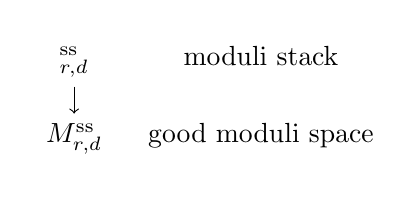
\begin{tikzpicture}
        \matrix (m) [matrix of math nodes, row sep=1em, column sep=1em]
        { \sM^{\text{ss}}_{r, d} & \text{moduli stack} \\ 
        M^{\text{ss}}_{r, d} & \text{good moduli space} \\};
        \path[->]
        (m-1-1) edge node[auto,swap] {$  $} (m-2-1)
        ;
        \end{tikzpicture}
        \end{center}
        \item $M^{\text{ss}}_{r,d}$ proper algebraic space
        \item Fibers are S-equiv. classes, so $M^{\text{ss}}_{r,d}$ parameterizes polystable sheaves.
    \end{itemize}
\end{columns}
\end{frame}

\subsection{Construction via a determinantal line bundle}
\begin{frame}[fragile]{Dim 1: Construction via a determinantal line bundle}
\pause
\begin{columns}[t]
    \column{0.5\textwidth}
    \begin{itemize}
        %\item<2-> $\sM^{\text{ss}}_{r,d}$ - stack of semistable vector bundles of $\rk r, \deg d$ on $C$
        %\item<3-> Stack-theoretic techniques $\Rightarrow$ $\sM^{\text{ss}}_{r,d}$ has a \textbf{good moduli space} $M^{\text{ss}}_{r,d}$ as a proper algebraic space.
        \item[]<1-> \textbf{Question}: Is $M^{\text{ss}}_{r,d}$ projective?
        \item[]<2-> {\footnotesize (Mumford: Yes, using GIT.)}
        \item<3-> Faltings: Ample determinantal line bundle.
        \item<4-> $\sE$ - universal bundle on $\sM^{\text{ss}}_{r,d} \times C$
        \item[]<5->
        \begin{center}
        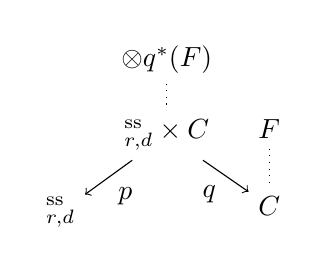
\begin{tikzpicture}
        \matrix (m) [matrix of math nodes, row sep=1em, column sep=1em]
        { & \sE \otimes q^*(F) & \\ 
        & \sM^{\text{ss}}_{r,d} \times C & F \\
        \sM^{\text{ss}}_{r,d} & & C \\};
        \path[dotted,-]
        (m-1-2) edge node[auto,swap] {$  $} (m-2-2)
        (m-2-3) edge node[auto,swap] {$  $} (m-3-3)
        ;
        \path[->] 
        (m-2-2) edge node[auto] {$ p $} (m-3-1)
        (m-2-2) edge node[auto,swap] {$ q $} (m-3-3)
        ;
        \end{tikzpicture}
        \end{center}
        \item<5-> For vector bundle $F$ with $\rk(F) = r', \det(F) = L$, set
        \[ \la_\sE(r', L) = \det(R p_* (\sE \otimes q^*F))^\vee \]
        \item<6-> Defines a group homomorphism
        \[ \la_\sE: K(X) \to \Pic(\sM^{\text{ss}}_{r,d}). \]
    \end{itemize}
    \pause
    
    \column{0.5\textwidth}
    \begin{itemize}
        \item<7-> Choose $r', L$ so that
        \[ \chi(C, E \otimes F) = 0 \text{ for } E \in \sM^{\text{ss}}_{r,d} \]
        \item<8-> (1) $\la_\sE(r', L)$ descends to $M^{\text{ss}}_{r,d}$ \\ (2) $R p_* (\sE \otimes q^*F)$ is a 2-term complex
        \[ [\sG_0 \xrightarrow{g} \sG_1], \quad \rk(\sG_0) = \rk(\sG_1). \]
        \item[]<9-> Global section of $\la_\sE(r', L)$: $s_F = \deg(g): \Oh \to \det(\sG_1) \otimes \det(\sG_0)^\vee$
        \item<10-> \textbf{Thm} (Faltings): For $E \in \sM^{\text{ss}}_{r,d}$ $\exists$ $F$ s.t.
        \[ H^0(X, E \otimes F) = H^1(X, E \otimes F) = 0 \]
        \onslide<11->{i.e. $s_F(E) \neq 0$ \pause $\Rightarrow$ $\la_\sE(r', L)$ is globally generated.}
        %\item<12-> \textbf{Thm} (Faltings): Given $C' \xrightarrow{\sE'} \sM^{\text{ss}}_{r,d}$, if $\deg(\la_\sE(r',L)|_{C'}) = 0$, then $\sE'$ is a family of S-equiv. sheaves. \\ \onslide<13->{$\Rightarrow$ Induced map $M^{\text{ss}}_{r,d} \to \p^N$ is finite, i.e. $\la_\sE(r',L)$ is ample.}
        \item<12-> \textbf{Thm} (Faltings): For any $C' \subs \sM^{\text{ss}}_{r,d}$, $\deg(\la_\sE(r',L)|_{C'}) > 0$
        \item[]<13->$\Rightarrow$ Induced map $M^{\text{ss}}_{r,d} \to \p^N$ is finite, i.e. $\la_\sE(r',L)$ is ample.
    \end{itemize}
\end{columns}
\end{frame}

\section{Dimension 2}
\subsection{Gieseker and Uhlenbeck moduli spaces}
\begin{frame}[fragile]{Dim 2: Gieseker and Uhlenbeck moduli spaces}
    \begin{itemize}
        \item<2->[] $X$ smooth, projective surface, $H \subs X$ very ample divisor
        \item<3->[] $v \in \Kn(X)$ class with $\rk(v) > 0$
        \item[]
    \end{itemize}
    
    \begin{columns}[t]
        \column{0.5\textwidth}
        \onslide<4->{\textbf{Gieseker stability}}
        \begin{itemize}
            \item<5-> Define stability using \textbf{reduced Hilbert polynomial}
            \[ p_E(n) = \frac{1}{\rk(E)} \chi(X, E(n H)) \]
            %\item<6-> HN- and JH-filtrations exist
            \item<7-> Good moduli space $M^{\text{Gies}}_v$ exists as a projective variety - constructed using GIT
            \item<8-> $M^{\text{Gies}}_v$ parameterizes polystable sheaves
            \item[]
            \item[]<16->
            \begin{center}
            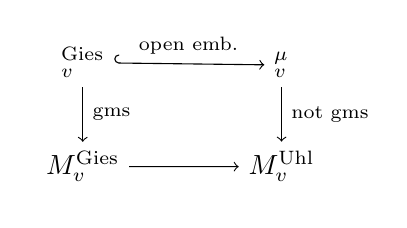
\begin{tikzpicture}
            \matrix (m) [matrix of math nodes, row sep=2em, column sep=4em]
            { \sM^{\mathrm{Gies}}_v & \sM^{\mu}_v \\
            M^{\mathrm{Gies}}_v & M^{\mathrm{Uhl}}_v \\};
            \path[right hook->] 
            (m-1-1) edge node[auto] {$ _\text{open emb.} $} (m-1-2)
            ;
            \path[->]
            (m-1-1) edge node[auto] {$ _\text{gms} $} (m-2-1)
            (m-1-2) edge node[auto] {$ _\text{not gms} $} (m-2-2)
            (m-2-1) edge node[auto] {$  $} (m-2-2)
            ;
            \end{tikzpicture}
            \end{center}
        \end{itemize}
        
        \column{0.5\textwidth}
        \onslide<4->{$\mu$-\textbf{stability}}
        \begin{itemize}
            \item<9-> Define stability using $H$-\textbf{slope}
            \[ \mu_H(E) = \frac{H \cdot c_1(E)}{\rk(E)} \]
            %\item<10-> HN- and JH-filtrations exist
            \item<11-> No good moduli space in general, but Uhlenbeck compactification comes close.
            \item<12-> $\mu_H$-semistable sheaves are torsion-free \\
            $\Rightarrow$ $E \subs E^{\vee\vee}$ and $\dim(E^{\vee\vee}/E) = 0$
            \item[]
            \item[]<13-> \textbf{Thm} (J. Li): Projective scheme $M^{\text{Uhl}}_v$ param. $\mu_H$-polystable sheaves up to:
            \begin{enumerate}
                \item<14-> isomorphic $E^{\vee\vee}$ 
                \item<15-> equal $l_p(E^{\vee\vee}/E)$ for all $p \in X$
            \end{enumerate}
        \end{itemize}
    \end{columns}
\end{frame}

\subsection{Bridgeland stability}
\begin{frame}{Dim 2: Bridgeland stability}
    \begin{columns}[t]
        \column{0.5\textwidth}
        \textbf{Fundamentals}
        \begin{itemize}
            %\item<2-> $X$ a smooth, projective variety
            \item<3-> Bridgeland (2003): generalize stability from $\Coh(X)$ to $D^b(X)$
            \item<4-> A \textbf{stability condition} is $\si = (\sA, Z)$:
            \begin{itemize}
                \item<5-> $\sA \subs D^b(X)$ heart of a t-structure \\
                \qquad\qquad (full abelian subcategory)
                \item<6-> $Z: \Kn(X) \to \C$ group hom.
                \item<7-> $Z(\sA) \in \Hb = \{ z \;|\; 0 < \phi(z) \le \pi \}$
            \end{itemize}
            \item<8-> $E \in \sA$ is \textbf{semistable} if for subobjects $F \subs E$,
            \[ \phi(Z(F)) \le \phi(Z(E)). \]
            \item<9-> \textbf{Thm} (Bridgeland): Stability conditions parameterized by a \textit{complex manifold} $\Stab(X)$. For fixed $v \in \Kn(X)$, wall-and-chamber structure on $\Stab(X)$.
            %\item<10-> If $\dim X = 1$, then $(\Coh(X), -\deg + i \rk) \in \Stab(X)$.
            %\item<11-> No $Z$ for $\sA = \Coh(X)$ if $\dim X \ge 2$.
            \item<11-> Existence is nontrivial -- $\Coh(X)$ doesn't work as $\sA$.
        \end{itemize}
        
        \column{0.5\textwidth}
        \textbf{Construction of stability conditions}
        \begin{itemize}
            %\item<12-> $(X,H)$ smooth, proj., polarized surface, $v \in \Kn(X)$
            \item<13-> Bridgeland, Arcara--Bertram: stability conditions on $X$ by \textit{tilting} $\Coh(X)$.
            \item<14-> For $\al, \be \in \R, \al > 0$, set
            \begin{align*}
                Z_{\al, \be}(E) & = \int_X e^{-(\al + \be i)H}\ch(E) \\
                \sA_\be & = \{ E \;|\; F \to E \to T[-1] \}
            \end{align*}
            where $\mu_H(F) \le \be < \mu_H(T)$ %$F, T \in \Coh(X)$ s.t. HN-factors satisfy $\mu_H(F_i) \le \be, \; \mu_H(T_i) > \be$. 
            \item<14-> \textbf{Thm} (B, AB): $(\sA_\be, Z_{\al,\be}) \in \Stab(X)$
            \item<15-> \textbf{Thm} (T, AHLH): Moduli stack $\sM^\si_v$ is algebraic, of finite type, universally closed, good moduli space $M^\si_v$ is a \textit{proper algebraic space}.
        \end{itemize}
    \end{columns}
\end{frame}

\subsection{{\color{purple} Vertical wall, projectivity, and Uhlenbeck}}
\begin{frame}[fragile]{Dim 2: Projectivity, vertical wall, and Uhlenbeck}
    \begin{columns}[t]
        \column{0.5\textwidth}
        \onslide<2->{\textbf{Question}: Is $M^\si_v$ projective?}
        \begin{itemize}
            \item<3-> Previously know cases (incomplete list):
            \begin{itemize}
                \item<4-> $X = \p^2, \p^1 \times \p^1, \text{Bl}_p \p^2$ - exceptional collections and quiver GIT.
                \item<5-> Gieseker stability for any $X$.
                \item<6-> $X = $ K3 or Enriques surface: relate to Gieseker by Fourier-Mukai.
            \end{itemize}
        \item<7-> \textbf{Thm} (BM): Determinantal line bundle $\sL_\si$ that is \textit{strictly nef} on $M^\si_v$: %$\exists \; w_\si \in K(X)$ s.t. $\sL_\si = \la_\sE(w_\si)$ 
        \item[] $\deg(\sL_\si|_C) > 0$ for $C \subs M^\si_v$
        \item<9-> $\Rightarrow$ If some $\sL_\si^{\otimes n}$ is globally generated, then $\sL_\si$ is ample!
        \item[]
        \item[]<10->
        \begin{center}
        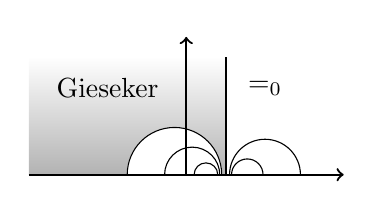
\begin{tikzpicture}[scale=0.5]

        %\shadedraw[bottom color=black!30!white,top color=white,draw=white] (-4,0) arc (180:0:2.49) -- (0,0) -- (1,0) -- (1,3.5) -- (-4,3.5);
        \shadedraw[bottom color=black!30!white,top color=white,draw=white] (-4,0) -- (-1.5,0) arc (180:0:1.2) -- (0,0) -- (1,0) -- (1,3) -- (-4,3);

        \draw[thick,->] (-4,0) -- (4,0) node[anchor=south east] {$\be$};
        \draw[thick,->] (0,0) -- (0,3.5) node[anchor=west] {$\al$};

        \draw[thick] (1,0) -- (1,3);


        %\draw[] (0.98,0) arc (0:180:2.49);
        %\draw[] (0.95,0) arc (0:180:1.8);
        \draw[] (0.9,0) arc (0:180:1.2);
        \draw[] (0.85,0) arc (0:180:0.7);
        \draw[] (0.8,0) arc (0:180:0.3);

        %\draw[] (1.02,0) arc (180:80:2);
        %\draw[] (1.05,0) arc (180:45:1.4);
        \draw[] (1.1,0) arc (180:0:0.9);
        \draw[] (1.15,0) arc (180:0:0.4);

        \draw (-2,2.2) node {Gieseker};
        \draw (2,2.2) node {$\be = \be_0$};
        %\fill (1,2) circle (0.04) node[anchor=east] {$\si$};

        \end{tikzpicture}
        \end{center}
        \end{itemize}
                
        \column{0.5\textwidth}
        \onslide<2->{\textbf{New affirmative case}: vertical wall}
        \begin{itemize}
            \item<10-> $(\al,\be)$-plane contains \textit{Gieseker chamber}, bounded by \textit{vertical wall} $\be = \be_0$.
            \item<12-> Polystable objects: $F \oplus (\oplus_i \Oh_{p_i}[-1])$, \\ $F$ $\mu_H$-polystable \textit{locally free}, and $p_i \in X$ \\ $\Rightarrow$ set-theoretic bijection with $M^{\text{Uhl}}_v$
            \item<13-> If $E \in \Coh(X)$ is $\mu_H$-stable but \textit{not locally free}, rotate $0 \to E \to E^{\vee\vee} \to Q \to 0$
            \[ \Rightarrow \quad E \; \overset{\text{S}}{\sim} \; E^{\vee\vee} \oplus Q[-1] \]
            \item[]<14-> \underline{\textbf{Thm} (T)}: On vertical wall:
            %\begin{itemize}
                \item[]<15-> $\sL_\si$ is ample and $M^\si(v)$ is projective.
                \item[]<16-> Bijective morphism $M^{\text{Uhl}}_v \to M^\si_v$.
            %\end{itemize}
            
            \item[]<17->
            \begin{center}
            \begin{tikzpicture}
            \matrix (m) [matrix of math nodes, row sep=2em, column sep=2em]
            { \sM^{\mathrm{Gies}}_v & \sM^{\mu}_v & \sM^\si_v \\
            M^{\mathrm{Gies}}_v & M^{\mathrm{Uhl}}_v & M^\si_v \\};
            \path[right hook->] 
            (m-1-1) edge node[auto] {$ _\text{open} $} (m-1-2)
            (m-1-2) edge node[auto] {$ _\text{open} $} (m-1-3)
            ;
            \path[->]
            (m-1-1) edge node[auto] {$ _\text{gms} $} (m-2-1)
            (m-1-2) edge node[auto] {$ $} (m-2-2)
            (m-1-3) edge node[auto,swap] {$ _\text{gms} $} (m-2-3)
            (m-2-1) edge node[auto] {$ $} (m-2-2)
            (m-2-2) edge node[auto] {$ _\text{bij.} $} (m-2-3)
            ;
            \end{tikzpicture}
            \end{center}
        \end{itemize}
    \end{columns}
\end{frame}

\subsection{Proof sketch \& questions}
\begin{frame}[fragile]{Dim 2: Proof sketch \& questions}
    \begin{columns}[t]
        \column{0.5\textwidth}
        \textbf{Proof sketch}
        \begin{itemize}
            \item<2-> %$\sM^\si_v$ quasi-comp. \& $\sL_\si$ strictly nef \\ $\Rightarrow$ 
            Enough to show: for $[E_0] \in \sM^\si_v$ there is $s \in \Ga(\sL_\si^{\otimes n})$ with $s(E_0) \neq 0$.
            \item<3-> Very special to vertical wall: there are curves $C \in |a H|$ and $F \in \Coh(C)$ s.t. $\sL_\si^{\otimes n} \cong \la_{j^* \sE}(F)^\vee$.
            %\item[]<3->
            %\begin{center}
            \begin{tikzpicture}
            \matrix (m) [matrix of math nodes, row sep=1em, column sep=1.5em]
            { & \sE & j^* \sE \\ 
            & \sM^\si_v \times X & \sM^\si_v \times C \\
            \sM^\si_v & X & C \\};
            \path[dotted,-]
            (m-1-2) edge node[auto,swap] {$  $} (m-2-2)
            (m-1-3) edge node[auto,swap] {$  $} (m-2-3)
            ;
            \path[left hook->]
            (m-2-3) edge node[auto] {$ j $} (m-2-2)
            (m-3-3) edge node[auto] {$ $} (m-3-2)
            ;
            \path[->] 
            (m-2-2) edge node[auto,swap] {$ $} (m-3-1)
            (m-2-2) edge node[auto] {$ $} (m-3-2)
            (m-2-3) edge node[auto] {$ $} (m-3-3)
            ;
            \end{tikzpicture}
            %\end{center}
            
            \item<4-> Step 1: for any $E \in \sM^\si_v$ and $C \in |a H|$,
            $H^i(C, F \otimes E|_C) = 0$ for $i \neq 0, 1$,
            \[ \dim H^0(C, F \otimes E|_C) = \dim H^1(C, F \otimes E|_C) \]
            $\Rightarrow$ $\la_{j^*\sE}(F)^\vee = \det[\sG_0 \xrightarrow{g} \sG_1]$ has section $s_F = \det(g)$.
        \end{itemize}
        
        \column{0.5\textwidth}
        \begin{itemize}
            \item<5-> Step 2: restriction theorems $\Rightarrow$ can choose $C \in |a H|$ s.t. $E_0|_C$ is a slope-semistable vector bundle
            \item<6-> Step 3: Faltings $\Rightarrow$ can choose $F \in \Coh(C)$ s.t. 
            \[ H^0(C, F \otimes E_0|_C) = H^1(C, F \otimes E_0|_C) = 0 \]
            $\Rightarrow$ $s_F(E_0) \neq 0$.
            \item<7-> $M^{\text{Uhl}}_v \to M^\si_v$ for free from Li's construction.
        \end{itemize}
        \onslide<8->{\textbf{Questions}}
        \begin{itemize}
            \item<9-> Is $M^{\text{Uhl}}_v \to M^\si_v$ isomorphism?
            \item<10-> Projectivity of other Bridgeland moduli spaces? For starters, is $\sL_{\si_\text{Gies}}$ relatively ample for $M^{\text{Gies}}_v \to M^\si_v$?
            \item<11-> Projectivity of other moduli of sheaves or complexes when GIT isn't available?
        \end{itemize}
    \end{columns}
\end{frame}

\section{Dimension 3}
\subsection{Work in progress: PT-stability}
\begin{frame}{Dim 3: PT-stability (work in progress)}
    \begin{columns}[t]
        \column{0.5\textwidth}
        \begin{itemize}
            \item<2-> $X$ smooth, projective 3-fold, $H \subs X$ very ample, $v \in \Kn(X)$ with $\rk(v) > 0$.
            \item<3-> A \textbf{PT-stable pair} is
            \[ \Oh_X \xrightarrow{f} F, \]
            $F$ pure dim 1, $\dim(\coker(f)) = 0$.
            \item<4-> (Bayer, Toda) Higher rank PT-pairs from \textit{polynomial/limit stability}. 
            \item<5-> PT-semistable $E \in D^b(X)$ satisfies
            \begin{itemize}
                \item<6-> $\sH^0(E)$ is $\mu_H$-semistable
                \item<6-> $\sH^1(E)$ is 0-dimensional
                \item<7-> $\Hom(T[-1], E) = 0$ if $\dim(T) = 0$
            \end{itemize}
            \item<8-> \textbf{Thm} (Lo): Moduli stack $\sM^{\text{PT}}_v$ is algebraic, of finite type, universally closed.
        \end{itemize}
        
        \column{0.5\textwidth}
        \begin{itemize}
            \item[]<9-> \underline{\textbf{Thm(ish)} (T)}: 
            %\begin{itemize}
                \item[]<10-> A determinantal line bundle $\sL$ on $\sM^{\text{PT}}_v$ is globally generated.
                \item[]<11-> Induced morphism $\pi: \sM^{\text{PT}}_v \to \p^N$ is injective on the locus of $\mu_H$-stable vector bundles.
            %\end{itemize}
            \item[]
            \item<12-> Global generation follows by restricting to curves.
            \item<13-> Questions:
            \begin{itemize}
                \item<14-> Does $\sM^{\text{PT}}_X(v)$ have a good moduli space? Is it projective?
                \item<15-> What does $\pi$ contract?
                \item<16-> Image of $\pi$ = analog of Uhlenbeck compactification for a 3-fold?
            \end{itemize}
            
        \end{itemize}
    \end{columns}
\end{frame}

\end{document}